% Scalar instruction entry source: tools/generate_scalar_instruction_catalog.py.
\subsection{\texttt{FGES}}
\label{sec:scalar-fges}
\index{FGES@\texttt{FGES}}
\begin{sloppypar}\noindent\textbf{Purpose.} Performs a signaling floating-point greater-than-or-equal comparison and writes 1 or 0 to RegDst.\end{sloppypar}\smallskip
\noindent\textbf{Syntax.}\par
\begin{lstlisting}[style=ptoscalarcode]
fges.{T} SrcL, SrcR, ->RegDst
\end{lstlisting}
\noindent\textbf{Encoding.}\par
\noindent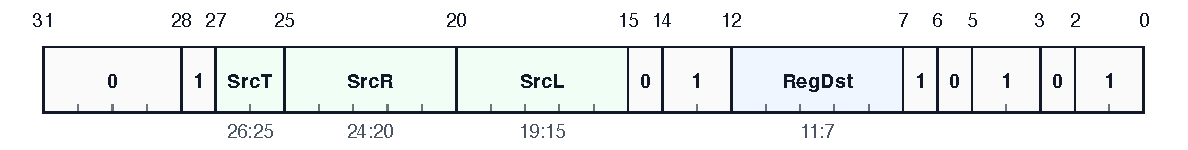
\includegraphics[width=\textwidth]{figs/encoding/scalar_instruction_entries/enc_fges.pdf}\par\smallskip
\begin{description}[leftmargin=0.18\linewidth,style=nextline]
\item[Format] \texttt{L32} \texttt{32-bit} scalar word.
\item[Pattern] \texttt{00001............011.....1011011}.
\end{description}
\noindent\textbf{Classification.}\par
\begin{description}[leftmargin=0.18\linewidth,style=nextline]
\item[Category] Floating-Point and Conversion.
\item[Family] Floating-point Compare.
\item[Execution class] \texttt{FSU}; uop\_kind=FSU.
\end{description}
\noindent\textbf{Operand fields.}\par
\begin{description}[leftmargin=0.18\linewidth,style=nextline]
\item[\texttt{RegDst}] Bits \texttt{11:7 (5b)}. 5-bit scalar destination register that receives the boolean compare result, encoded as 1 for true and 0 for false; X0 discards the write.
\item[\texttt{SrcL}] Bits \texttt{19:15 (5b)}. 5-bit scalar source register holding the left or only floating-point/conversion operand; SrcType or the assembly suffix determines the interpreted format.
\item[\texttt{SrcR}] Bits \texttt{24:20 (5b)}. 5-bit scalar source register holding the right floating-point operand.
\item[\texttt{SrcType}] Bits \texttt{26:25 (2b)}. 2-bit source format selector for floating-point or conversion operands. The assembly suffix \{T\} names the selected floating-point element format.
\end{description}
\noindent\textbf{Operation.}\par
\begin{lstlisting}[style=ptoscalarcode]
a = Read(SrcL)  // fd: full 64b; fs: low 32b
b = Read(SrcR)
// SrcType selects fd/fs; NaNs make predicate false
result = OrderedGe(a, b) ? 1 : 0
Write(RegDst, result)
\end{lstlisting}
\Needspace{0.08\textheight}
